\section{Decomposition 2: OtherFunctionality1 (M1, P2, UC11)}

\subsection{Module to decompose}
    In this run we decompose OtherFunctionality1.


\subsection{Selected architectural drivers}
    The non-functional drivers for this decomposition are:
    \begin{itemize}
    	\item \emph{M1}: Integrate new sensor or actuator manufacturer
        \item \emph{P2}: Requests to the pluggable data database
    \end{itemize}

    The related functional drivers are:
    \begin{itemize}
        \item \emph{UC11}: Send pluggable device data (P2) \\
              This use case stores pluggable device data in the pluggable device data storage.
              This could be a sensor reading or an actuator status.
    \end{itemize}

    \paragraph{Rationale}
    We chose M1 as it was one of the remaining quality attributes with high priority.
    M1's focus on easily introducing new types of devices to the system is very important
    because of the fast growing market for IoT and development of applications for IoT.
    Thus, we want to handle this quality attribute before U2 (the other remaining
    attribute with high priority), as we presume that customer organisations
    are more interested in using new devices than the effort it takes for
    infrastructure owners to install the devices. \\
    We also chose P2 because it is strongly related to M1; the whole data flow from
    devices to storage/applications needs to exist before modifications can even be made.
    This combination of M1 and P2 would force us to handle processing and
    storage of data while making the involved components as simple as possible to modify.


\subsection{Architectural design}
    This section describes what needs to be done to satisfy the requirements for
    this decomposition and how involved problems/obstacles are solved.

    \paragraph{M1: Data conversion}
        With new types of devices, the pluggable data processing subsystem
        should be extended with relevant data conversions,
        e.g. converting temperature in degrees Fahrenheit to degrees Celsius. \\
        The \texttt{DeviceDataConverter} is put in place to handle the
        task of converting pluggable device data to data of a different type in the system.
        This component can easily be modified for new types of data simply by
        adding a new conversion method for the new.

    \paragraph{M1: Usage of new data by applications}
        The available applications in the system can be updated to use any
        new pluggable devices. \\
        This is made possible by the RequestData
        interface provided by \texttt{DeviceDataScheduler}.
        Data of the new type of device can be requested in the same way
        as for older devices: by using the device's unique id.
        The application manager can get pluggable device data from the
        \texttt{PluggableDeviceDataDB} and return this data to applications in
        the DeviceData datatype. This datatype can easily be
        updated for new types of pluggable devices.

    \paragraph{P2: Scheduling}
        The pluggable data processing subsystem needs to be able to run in normal
        or overload mode, depending on whether or not the system can process
        requests within the deadlines given in the quality requirement. Also,
        a mechanism should be in place to avoid starvation of any type of request. \\
        The \texttt{DeviceDataScheduler} is used to deal with this problem.
        It is responsible for scheduling requests that wish to interact with
        the \texttt{PluggableDeviceDataDB}. In normal mode, the system processes
        incoming requests in a FIFO order. In overload mode, the requests are
        given a priority based on what the request is for and what the source
        of the request is. The requests are then not simply processed in an
        order based on their priorities, but an aging technique is to be used
        such that starvation will be avoided. Thus, in overload mode,
        requests are processed in an order based on a combination of the
        priorities of the requests and the age of the requests.

    \paragraph{P2: Pluggable data separation}
        The processing of (large amounts of) requests concerning pluggable
        data has no impact on requests concerning other data, e.g. available applications. \\
        In order to statisfy this constraint, all data directly related to
        pluggable data has been separated into the \texttt{PluggableDeviceDataDB}.
        All requests concerning pluggable data will be handled by this new
        component. \texttt{PluggableDeviceDataDB} will run on a node different
        from the node that the \texttt{Datbase} component runs on. This way
        requests concerning pluggable will have no impact on
        requests concerning other data.

    \paragraph{M1: Handling new types of pluggable devices}
        The new types of sensor or actuator data should be transmitted,
        processed and stored, and should be made available to applications.
        The infrastructure managers must be able to initialize the new type
        of pluggable device, configure access rights for these devices, and
        view detailed information about the new type of pluggable device. \\
        The components created thus far have been created with high cohesion in
        mind so that updating them for new devices would be relatively straightforward.
        In order for this constraint to be satisfied, changes have to be made to
        the following elements:
        \begin{itemize}
            \item \emph{PluggableDeviceFacade}: This component needs to be updated
                  so that the new type of device can be initialised and configured,
                  and thus so that the device's data can be sent to the system.
            \item \emph{DeviceData}: Depending on how this data type
                  is implemented, it might need an update in order for it
                  to represent possible new data types (for example
                  Temperature Filipcikova) and for the new data types to be
                  serialized.
            \item \emph{PluggableDeviceDataDB}: The database needs to be updated
                  so that information can be retrieved about the new types
                  of sensors and the new types of data. Data related to the
                  displaying of sensor data will also need to be updated.
            \item \emph{PluggableDeviceConverter}: see above.
        \end{itemize}


\subsection{Instantiation and allocation of functionality}
    This section describes the new components which instantiate our solutions described
    in the section above and how components are deployed on physical nodes. \\
    Unless stated otherwise the responsibilities assigned in the first decomposition are unchanged.

    \paragraph{Decomposition}
        Figure \ref{fig:it2-cc_main} shows the components resulting from the
        decomposition in this run.

        \begin{figure}[!h]
        	\centering
            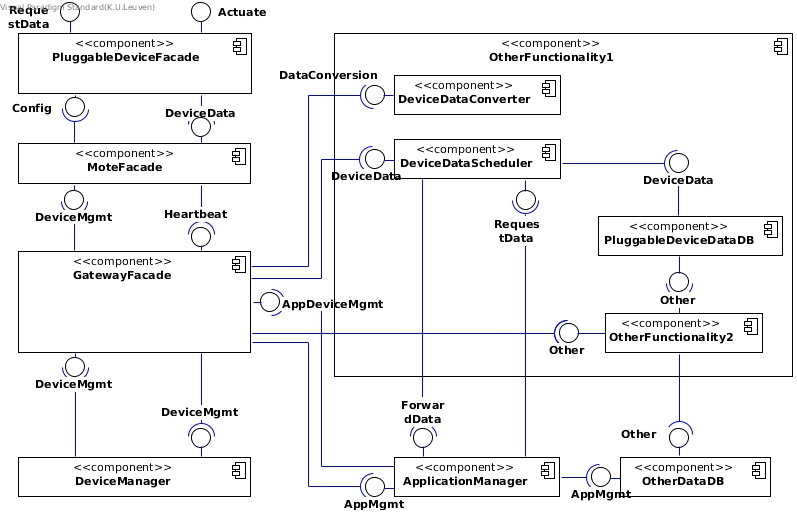
\includegraphics[width=1\textwidth]{images/component-diagram-2}
        	\caption{Component-and-connector diagram of this decomposition.}
            \label{fig:it2-cc_main}
        \end{figure}

        The responsibilities of the components are as follows:

    \subparagraph{DeviceDataConverter}
        The \texttt{DeviceDataConverter} is resposible for converting
        pluggable device data in the data processing subsystem. (M1)

    \subparagraph{DeviceDataScheduler}
        Responsible for scheduling incoming read and write requests for
        pluggable device data. Monitors throughput of requests and switches
        between normal and overload mode when appropriate. Avoids starvation
        of any type of request. (P2)

    \subparagraph{PluggableDeviceDataDB}
        Database dedicated to pluggable device data. (P2)

    \subparagraph{PluggableDeviceFacade}
        Responsible for sending pluggable device data to \texttt{MoteFacade}.
        Needs to be initialised in order for the data to be used/stored. (UC11)

    % \paragraph{Behaviour}
        % A SEQUENCE DIAGRAM WOULD BE USEFUL FOR
        % UC11: shows how the gateway checks if devices are initialised

    \paragraph{Deployment}
        Figure \ref{fig:it2-depl_main} shows the allocation of components
        to physical nodes.

        \begin{figure}[!h]
        	\centering
        	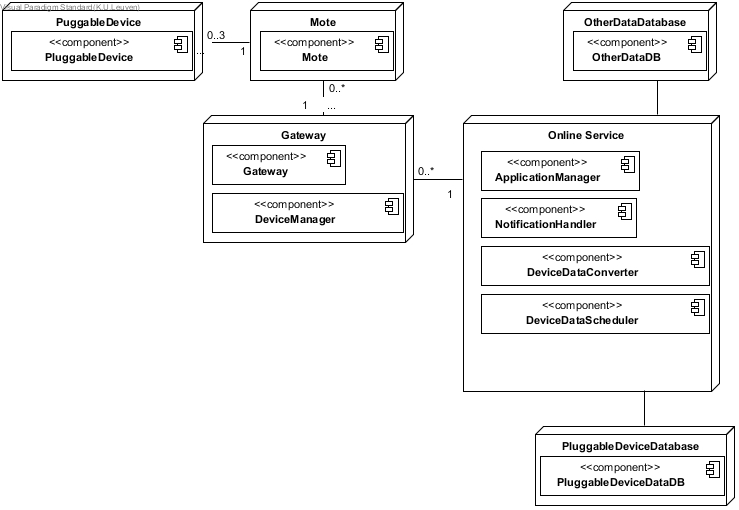
\includegraphics[width=0.8\textwidth]{images/deployment-diagram-2}
        	\caption{Deployment diagram of this decomposition.
        	}\label{fig:it2-depl_main}
        \end{figure}


\subsection{Interfaces for child modules}\label{add2-interfaces}
    This section describes the interfaces assigned to the components defined
    in the section above. Per interface, we list its methods by means of its
    syntax. The data types used in these interfaces are defined in the following section. \\

    Each method shows which (part of a) quality attribute or use case caused
    a need for the method. However, this does not mean that a method is
    only to be used to satisfy that quality  attribute or use case, it could
    be used for other causes not yet mentioned here.

    The interfaces and methods defined here are to be seen as an
    extension of the interfaces defined in previous sections, unless
    explicitly stated otherwise.

    \subsubsection{ApplicationManager}
        \begin{itemize}
            \item ForwardData
            \begin{itemize}
                \item \texttt{void rcvData(PluggableDeviceID pID, DeviceData data)}
                    \begin{itemize}
                        \item Effect: Sends pluggable device data to an application that wants to use it
                        \item Created for: UC11: system relays data to applications
                    \end{itemize}
                \item \texttt{List<int> getApplicationsForDevice(PluggableDeviceID pID)}
                    \begin{itemize}
                        \item Effect: Returns a list of application instances that can use the device with id "pID".
                        \item Created for: UC11: the system looks up the list of applications that use the pluggable device
                    \end{itemize}
            \end{itemize}
        \end{itemize}

    \subsubsection{Database}
        \begin{itemize}
            \item AppMgmt
            \begin{itemize}
                \item \texttt{List<int> getApplicationsForDevice(PluggableDeviceID pID)}
                    \begin{itemize}
                        \item Effect: Returns a list of applications that can use the device with id "pID".
                        \item Created for: UC11: the system looks up the list of applications that use the pluggable device
                    \end{itemize}
            \end{itemize}
        \end{itemize}


    \subsubsection{GatewayFacade}
        \begin{itemize}
            \item DeviceData, last defined in section \ref{add1-interfaces}
            \begin{itemize}
                \item \texttt{void rcvData(PluggableDeviceID pID, DeviceData data)}
                    \begin{itemize}
                        \item Now (also) used by: UC11 \\
                              P2: storing new pluggable data
                    \end{itemize}
                \item \texttt{void rcvDataCallback(PluggableDeviceID pID, DeviceData data, int requestID)}
                    \begin{itemize}
                        \item Now (also) used by: UC11 \\
                              P2: storing new pluggable data
                    \end{itemize}
            \end{itemize}

            \item DeviceMgmt, last defined in section \ref{add1-interfaces}
            \begin{itemize}
                \item \texttt{void setConfig(PluggableDeviceID pID, Map<String,String> config)}
                \begin{itemize}
                    \item Effect: Set the given configuration parameters of a
                          PluggableDevice to the given values. Setting unknown parameters
                          on a PluggableDevice has no effect.
                    \item Created for: UC11: pluggable device needs to be initialised \\
                          M1: pluggable device must be able to be initialised
                \end{itemize}
            \end{itemize}
        \end{itemize}

    \subsubsection{MoteFacade}
        \begin{itemize}
            \item DeviceData
            \begin{itemize}
                \item \texttt{void rcvData(PluggableDeviceID pID, DeviceData data)}
                    \begin{itemize}
                        \item Effect: Propagates pluggable device data to
                              the connected gateway by call rcvData on the gateway.
                              (Initiated by the device).
                        \item Created for: UC11 \\
                              P2: storing new pluggable data
                    \end{itemize}
                \item \texttt{void rcvDataCallback(PluggableDeviceID pID, DeviceData data, int requestID)}
                    \begin{itemize}
                        \item Effect: Propagates pluggable device data to the
                              connected gateway by calling rcvData on the gateway.
                              (Callback of getDataAsync).
                        \item Created for: UC11 \\
                              P2: storing new pluggable data
                    \end{itemize}
            \end{itemize}

            \item DeviceMgmt, last defined in section \ref{add1-interfaces}
            \begin{itemize}
                \item \texttt{void setConfig(PluggableDeviceID pID, Map<String,String> config)}
                \begin{itemize}
                    \item Effect: Set the given configuration parameters of a
                          PluggableDevice to the given values. Setting unknown parameters
                          on a PluggableDevice has no effect.
                    \item Created for: UC11: pluggable device needs to be initialised \\
                          M1: pluggable device must be able to be initialised
                \end{itemize}
            \end{itemize}
        \end{itemize}

    \subsubsection{PluggableDeviceFacade}
        \begin{itemize}
        	\item Config
        	\begin{itemize}
                \item \texttt{Map<String,String> getConfig()}
                    \begin{itemize}
                        \item Effect: Returns the current configuration of a
                              pluggable device as a parameter-value map.
                        \item Created for: Given constraint, unused at the moment.
                    \end{itemize}
                \item \texttt{boolean setConfig(Map<String,String> config)}
                    \begin{itemize}
                        \item Effect: Set the given configuration parameters of the
                              pluggable device to the given values. Setting unknown parameters
                              on a pluggable device (e.g., ‘noise threshold’ → ‘3’ on a light
                              sensor) has no effect.
                        \item Created for: Given constraint \\
                              UC11: pluggable device needs to be initialised \\
                              M1: pluggable device must be able to be initialised
                    \end{itemize}
        	\end{itemize}

        	\item RequestData
        	\begin{itemize}
                \item \texttt{DeviceData getData()}
                    \begin{itemize}
                        \item Effect: Synchronously retrieve the device data of a device.
                        \item Created for: Given constraint, unused at the moment.
                    \end{itemize}
                \item \texttt{void getDataAsync(int requestID)}
                    \begin{itemize}
                        \item Effect: Asynchronously retrieve the device data
                              of a device (by calling rcvDataCallback).
                        \item Created for: Given constraint, unused at the moment.
                    \end{itemize}
        	\end{itemize}

        	\item Actuate
        	\begin{itemize}
                \item \texttt{void sendActuationCommand(String commandName)}
                    \begin{itemize}
                        \item Effect:
                        \item Created for: Given constraint, unused at the moment.
                    \end{itemize}
        	\end{itemize}
        \end{itemize}

    \subsubsection{DeviceManager}
        \begin{itemize}
        	\item DeviceMgmt, last defined in section \ref{add1-interfaces}
        	\begin{itemize}
        		\item \texttt{bool isDeviceInitialised(PluggableDeviceID pID)}
        		\begin{itemize}
        			\item Effect: Returns true if the device with id "pID" has been initialized.
                    \item Created for: UC11: pluggable device needs to be initialised \\
                          M1: pluggable device must be able to be initialised
                    \item TODO: need this check? is 'initialized' status stored in DB or on gateways? or both?
        		\end{itemize}
        	\end{itemize}
        \end{itemize}

    \subsubsection{DeviceDataConverter}
    \begin{itemize}
        \item DataConversion
        \begin{itemize}
            \item \texttt{DeviceData convert(PluggableDeviceID pID, DeviceData data, string type)}
            \begin{itemize}
                \item Effect: Converts pluggable device data into other pluggable device
                      data that contains the same information in a different type
                \item Created for: M1: data processing subsystem should be
                      extended with relevant data conversions
            \end{itemize}
        \end{itemize}
    \end{itemize}

    \subsubsection{DeviceDataScheduler}
        \begin{itemize}
            \item RequestData
            \begin{itemize}
                \item \texttt{List<DeviceData> getData(int applicationID, PluggableDeviceID pID, DateTime from, DateTime to)}
                \begin{itemize}
                    \item Effect: Requests data from a specific device in a certain time period
                    \item Created for: P2: requests from applications
                \end{itemize}
            \end{itemize}

            \item DeviceData
            \begin{itemize}
                \item \texttt{void rcvData(PluggableDeviceID pID, DeviceData data)}
                    \begin{itemize}
                        \item Effect: Sends pluggable device data to the scheduler to be processed.
                        \item Created for: UC11 \\
                              P2: storing new pluggable data
                    \end{itemize}
            \end{itemize}
        \end{itemize}

    \subsubsection{PluggableDeviceDataDB}
        \begin{itemize}
            \item DeviceData
            \begin{itemize}
                \item \texttt{void rcvData(PluggableDeviceID pID, DeviceData data)}
                \begin{itemize}
                    \item Effect: Sends pluggable device data to the DB to be stored.
                    \item Created for: UC11 \\
                          P2: storing new pluggable data
                \end{itemize}
                \item \texttt{List<DeviceData> getData(PluggableDeviceID pID, DateTime from, DateTime to)}
                \begin{itemize}
                    \item Effect: Returns data from a specific device in a certain time period.
                    \item Created for: P2: lookup queries
                \end{itemize}
            \end{itemize}
        \end{itemize}


\subsection{Data type definitions}
    This section defines new data types that are used in the interface descriptions above.

    \paragraph{DeviceData}
               contains data from a pluggable device at a certain point in time
               (value, type, date) (e.g. a sensor reading, an actuator status)
    \paragraph{PluggableDeviceSettings}
              contains settings for a pluggable device (power status,
              data update rate, ...)
    \paragraph{DateTime}
               Represents an instant in time, typically expressed as a date and time of day.
    \paragraph{PluggableDeviceID}
               A unique identifier of the \texttt{PluggableDevice}
    \paragraph{Map<String,String>}
               is a map of key-value pairs.  E.g., ‘sensitivity’→‘10’.


\subsection{Verify and refine}
    The selected architectural drivers have been handled completely
    in this decomposition.
    This section describes per component which (parts of) the remaining
    requirements it is responsible for. If requirements are split in
    multiple parts, this is indicated by the addition of a letter
    (or number, depending on the structure of the requirement) after their title.

    \paragraph{ApplicationManager}
        \begin{itemize}
            \item \emph{Av2}: Application failure \\
                   Prevention: a, b \\
                   Detection: a, b, c \\
                   Resolution: a, b, c
           \item \emph{P1}: Large number of users: c
           \item \emph{M2}: Big data analytics on pluggable data and/or application usage data: d, e
           \item \emph{U1}: Application updates: a, b, c, d
           \item \emph{U2}: Easy Installation: e
           \item \emph{UC12}: Perform actuation command
           \item \emph{UC17}: Activate an application: 3, 4
        \end{itemize}

    \paragraph{Database}
        \begin{itemize}
          	\item None
        \end{itemize}

    \paragraph{GatewayFacade}
        \begin{itemize}
            \item \emph{Av1}: Communication between SIoTIP gateway and Online Service \\
                               Resolution: b, c, d
            \item \emph{U2}: Easy Installation: a, c, d
        \end{itemize}

    \paragraph{MoteFacade}
        \begin{itemize}
            \item \emph{U2}: Easy Installation: b, c, d
            \item \emph{UC04}: Install mote: 1, 2
            \item \emph{UC05}: Uninstall mote: 1
            \item \emph{UC06}: Insert a pluggable device into a mote: 2
            \item \emph{UC07}: Remove a pluggable device from its mote: 2
        \end{itemize}

    \paragraph{NotificationHandler}
        \begin{itemize}
            \item \emph{UC16}: Consult notification message: 5
            \item \emph{UC17}: Activate an application: 5, 6
        \end{itemize}

    \paragraph{OtherFunctionality2}
        \begin{itemize}
            \item \emph{Av1}: Communication between SIoTIP gateway and Online Service \\
                               Detection: a, b, c, d
                               Resolution: a
           	\item \emph{P1}: Large number of users: a
            \item \emph{M2}: Big data analytics on pluggable data and/or application usage data: a
            \item \emph{U2}: Easy Installation: e
            \item \emph{UC01}: Register a customer organisation
            \item \emph{UC02}: Register an end-user
            \item \emph{UC03}: Unregister an end user
            \item \emph{UC04}: Install mote: 3
            \item \emph{UC05}: Uninstall mote: 2.b
            \item \emph{UC06}: Insert a pluggable device into a mote: 3: topology part; alternative 3a.1.b
            \item \emph{UC07}: Remove a pluggable device from its mote: 3.b
            \item \emph{UC08}: Initialise a pluggable device: 1, 2, 4
            \item \emph{UC09}: Configure pluggable device access rights
            \item \emph{UC10}: Consult and configure the topology
            \item \emph{UC13}: Configure pluggable device
            \item \emph{UC16}: Consult notification message: 1, 2, 3, 4
            \item \emph{UC17}: Activate an application: 1, 2
            \item \emph{UC19}: Subscribe to application
            \item \emph{UC20}: Unsubscribe from application
            \item \emph{UC21}: Send invoice
            \item \emph{UC22}: Upload an application
            \item \emph{UC23}: Consult application statistics
            \item \emph{UC24}: Consult historical data
            \item \emph{UC25}: Access topology and available devices
            \item \emph{UC26}: Send application command or message to external front-end
            \item \emph{UC27}: Receive application command or message to external front-end
            \item \emph{UC28}: Log in
            \item \emph{UC29}: Log out
        \end{itemize}

    \paragraph{PluggableDeviceDataDB}
        \begin{itemize}
            \item \emph{M2}: Big data analytics on pluggable data and/or application usage data: b
        \end{itemize}

    \paragraph{PluggableDeviceFacade}
        \begin{itemize}
        	\item \emph{U2}: Easy Installation: d
        \end{itemize}

    \paragraph{DeviceManager}
        \begin{itemize}
            \item \emph{U2}: Easy Installation: c, d
            \item \emph{UC04}: Install mote: 4
            \item \emph{UC05}: Uninstall mote: 2
            \item \emph{UC06}: Insert a pluggable device into a mote: 3: uninitialised part; alternative 3a.1 3a.2 3a.4; 4
            \item \emph{UC07}: Remove a pluggable device from its mote: 3.a, 3.c
            \item \emph{UC08}: Initialise a pluggable device: 3,
        \end{itemize}

    \paragraph{DeviceDataScheduler}
        \begin{itemize}
            \item \emph{P1}: Large number of users: b
            \item \emph{M2}: Big data analytics on pluggable data and/or application usage data: b, c
        \end{itemize}
